\chapter{Evaluation}
This chapter presents the results of the evaluation of our approach. The experiments have been conducted based on several test parameters and their combinations and we will be analyzing the baseline parameter sets as well as the key combinations. 

The capacity estimation tools can face different challenges in real networks. We will try to imitate some of these challenges in our custom-built emulated network and find out what kind of impact can they have on measurement accuracy.\\
Two of the biggest obstacles our framework has to face are the cross-traffic and the \sc{ICMP} rate limiting, which we will discuss shortly in respective sections.

Overall, we will evaluate the tool based on the path length, the capacity range, the packet size, the packet train length. For a deeper insight we will also apply the ICMP rate limiting and also check the influence of the packet loss on accuracy. 
The tests are conducted on an empty network as well as with the significant amount of cross-traffic load.

The following are the parameters which we use for the evaluation of the tool. They are manually configured by us for each test suite in order to get a better picture about the quality of our approach and shows us whether it is applicable in real life:
\begin{itemize}
	\item \textbf{Path Length} - the number of routers between the source host and the destination host. (i.e. number of hops minus one)
	\\ The default value: 8 routers.
	\item \textbf{Capacity Range} - The range of numbers from which a capacity for each link will be generated
	\\ The default value: [10, 100).
	\item \textbf{Packet Size} - The size of each packet that will be sent from the source host to the destination. It represents the total size of the packet including TCP and IP headers(each weighing 20 bytes). 
	\\ The default value: 1500 bytes (i.e. size of MSS + TCP header + IP header = 1460 + 20 + 20)
	\item \textbf{Packet Train Length} - The amount of packets that will be targeted at each hop
	\\ The default value: 300 packets.
	\item \textbf{Packet Loss} - The emulated packet loss on each router.
	\\ The default value: 0.
	\item \textbf{ICMP Rate Limit} - The artificial ICMP rate limit that will be assigned to each router. 
	\\ The default value: 0.
	\item \textbf{Cross Traffic} - The coefficient of the cross traffic load. The Optimal value is recommended to be assigned from 0 to 1.0, the value of 0 meaning an empty network without any cross traffic. 
\end{itemize}

To ensure the reliability on the the test results, we conduct test runs with each test configuration 20 times.

\section{Test Environment and Setup}
For the testing purposes we decided to build a virtual network using the network emulator - Mininet\cite{mnHome}. It provides the necessary tools to create an artificial network and has a very handy Python API that enables us to build custom topologies.


The figure \ref{topology} represents the template of the network that we have used in our experiments. It consists of the source and the destination hosts, the top and the bottom hosts and the routers that connect them with each other. 

\begin{figure}[h]
 \centering
	 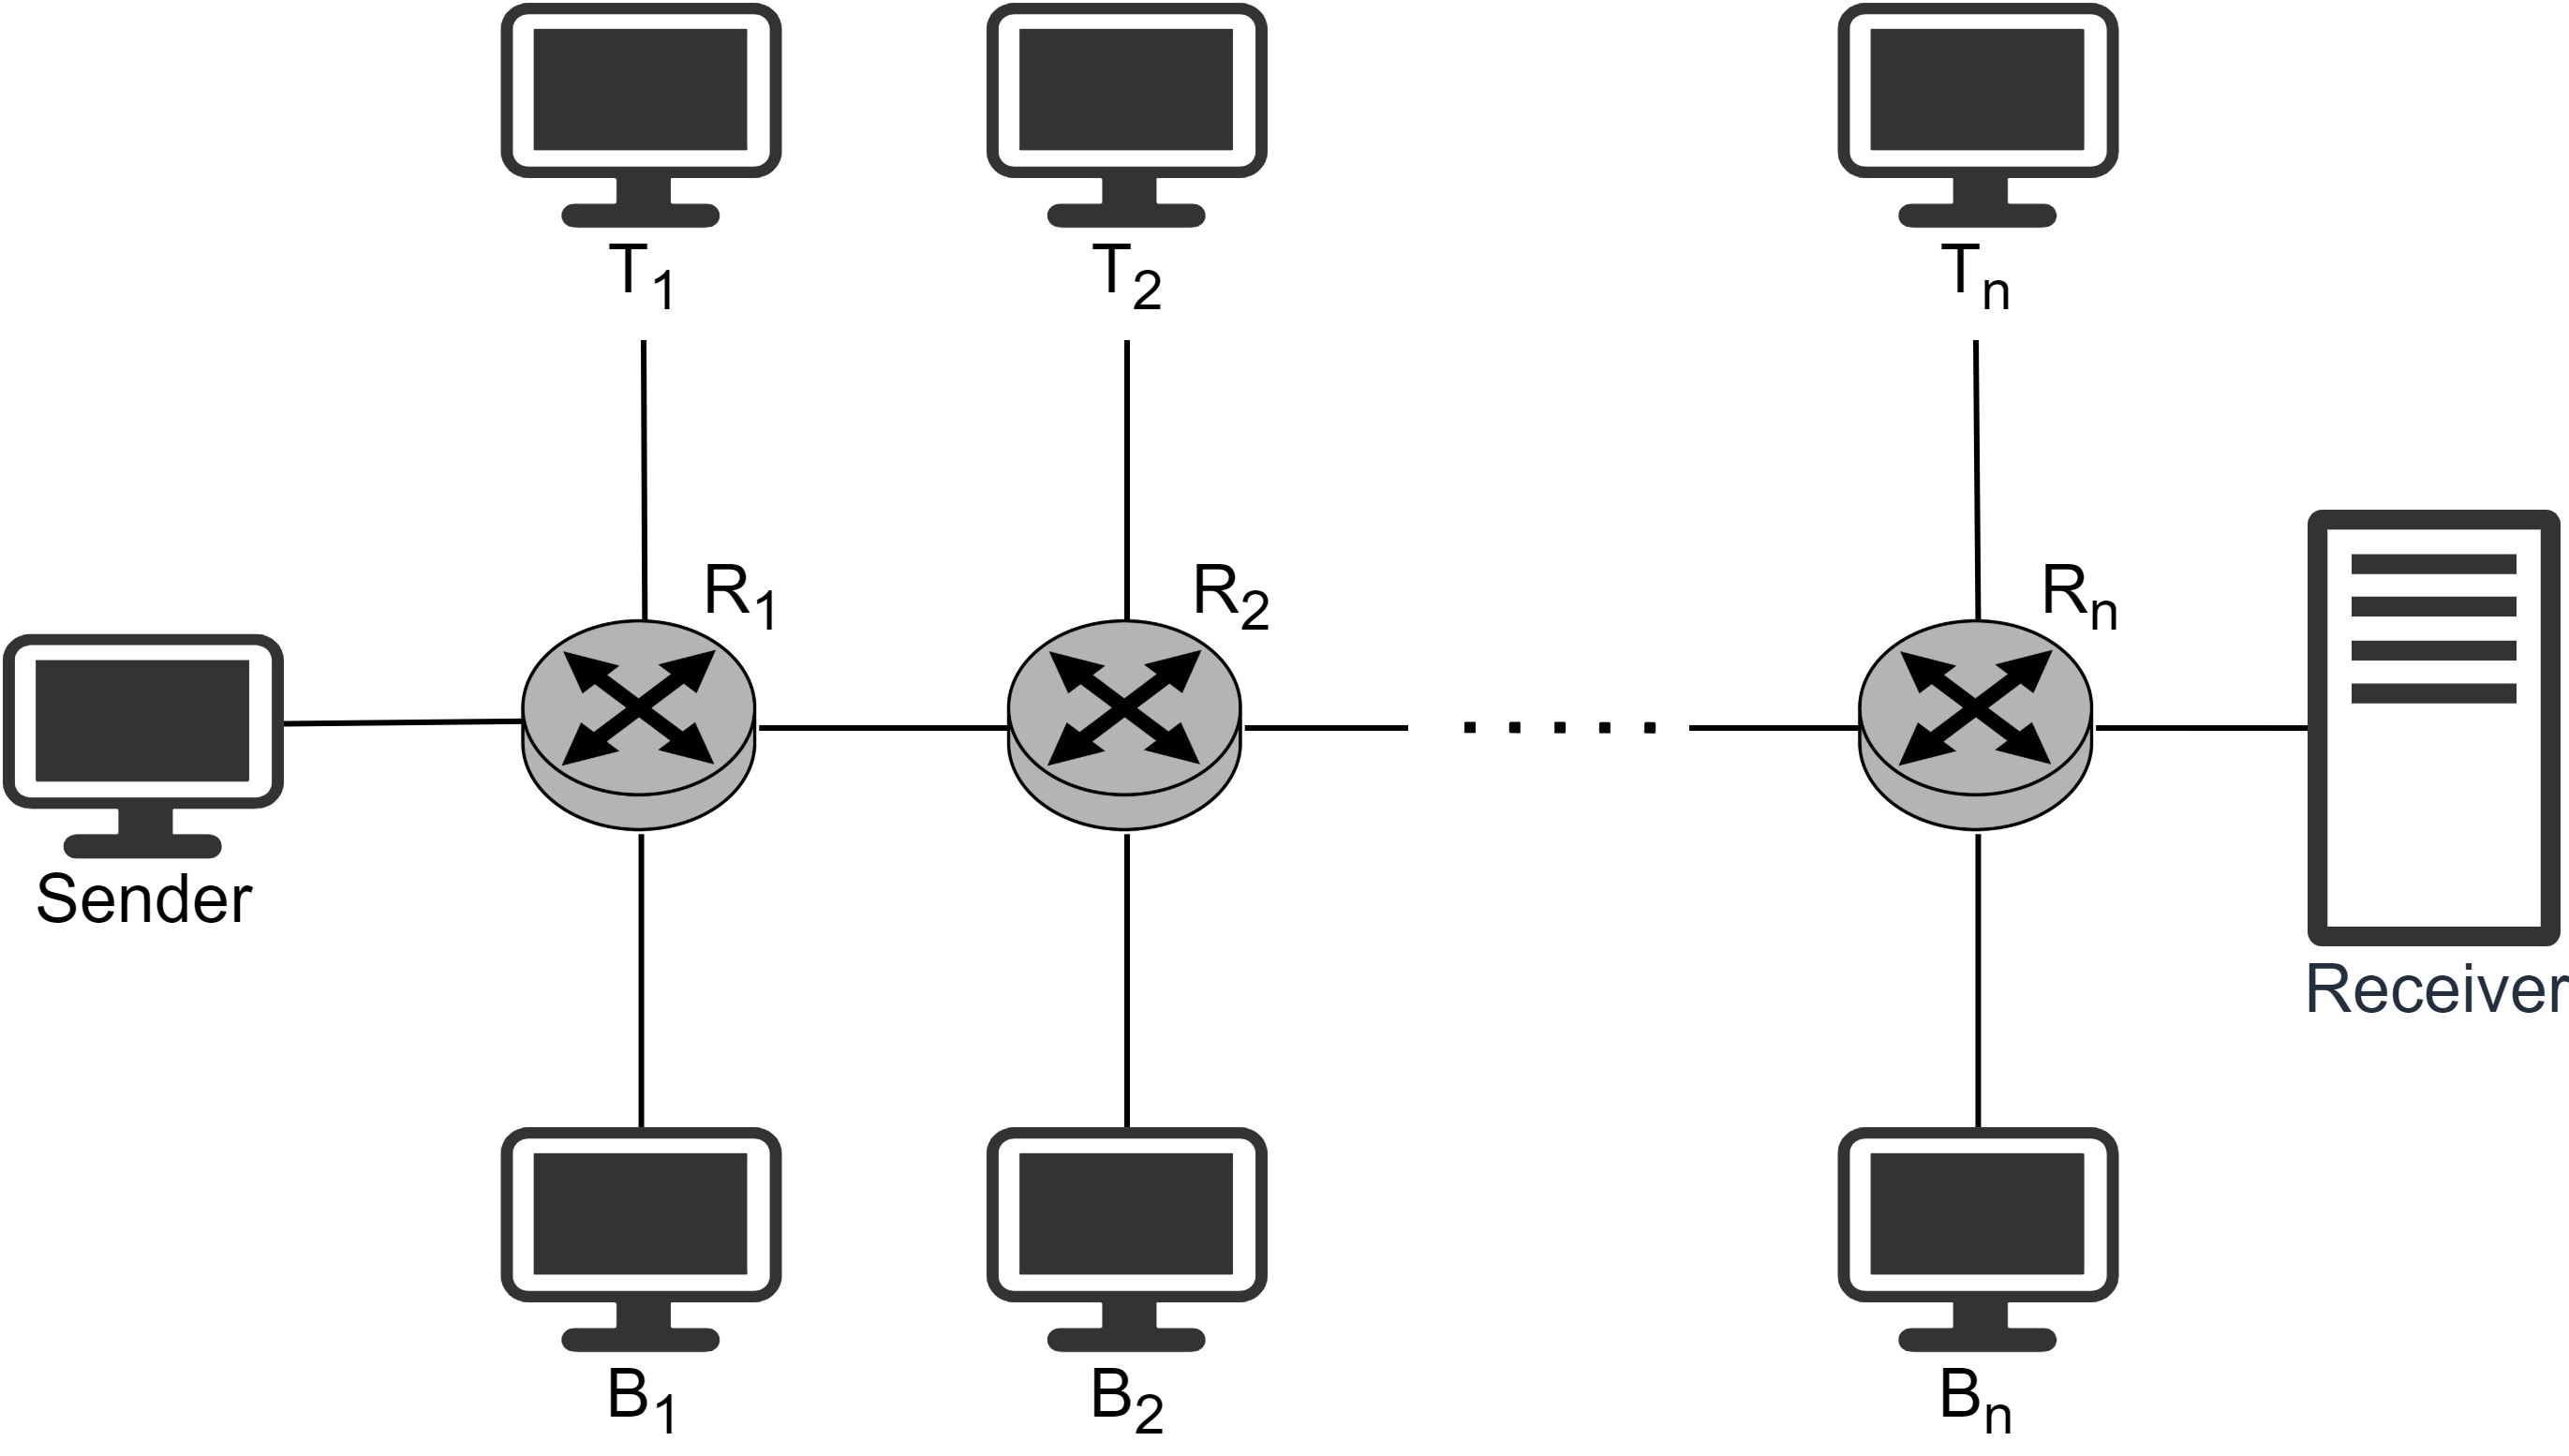
\includegraphics[width=\textwidth]{topology}
 \caption{The template network topology}
 \label{topology}

\end{figure}

As a reader can see from the Figure \ref{topology}, the main hosts (sender and receiver) are connected with a sequence of \texttt{n} routers, each consisting of four interfaces and each having its own subnetwork. The number of routers and, therefore, the number of top and bottom hosts is dynamic and configurable. The routes from and to all hosts are statically configured.

The measurements are conducted based on the main path, which is the one that consists of the routers \texttt(1...n) and connects the sender to the receiver. The top and the bottom hosts are used for generating cross-traffic in later experiments. The cross-traffic interferes with the main flow of packets and has a significant influence on the accuracy of capacity estimations.

The measuring node is the "Sender", as using our tool only makes sense if the measuring node is the one that generates the traffic. All the necessary traffic is captured at this node with the \texttt{tcpdump} command and subsequently analyzed by our program that delivers the final result.

Finally, it is also important to mention that Mininet has certain limitations, namely, it is limited with the computational power of the machine it runs on. Therefore, we have decided to execute the estimation experiments on the testbed of the chair.

\textbf{Disclaimer:} As the routers are all configured the same way in terms of packet loss and \sc{ICMP} rate limiting, the results from all hops are analyzed together. The tests have shown no difference between the accuracy rates of different indexes of hops, e.g. the accuracy rate of the capacity estimations from the source to R\textsubscript{1} and to R\textsubscript{n} is practically the same in equal circumstances.

\section{Evaluation in Empty Network}
\label{empty_net}
We decided to divide our evaluation into two parts: the section \ref{empty_net} describes the measurement results on an empty network and the section \ref{section_ct} analyzes the effect of the cross traffic based on the experiment outcomes on an overloaded network where the flow of our generated traffic is interfered by the cross-traffic. 

To have a broad picture of the initial results, we first conducted baseline measurements with the default configuration of the parameters, namely, the path length of 8 routers and the packet size of 1500 bytes in a capacity range of [10, 100), which resulted in accurate estimations. 
\\The graph in the figure \ref{baseline} represents the comparison between the real and estimated capacities and as one can see, the accuracy is high.\\
Moreover, the figure \ref{baseline_error} and the table \ref{baseline_error_stats} represent the error rate of the baseline measurement and statistical details about error rates respectively.

\begin{figure}[H]
 \centering
 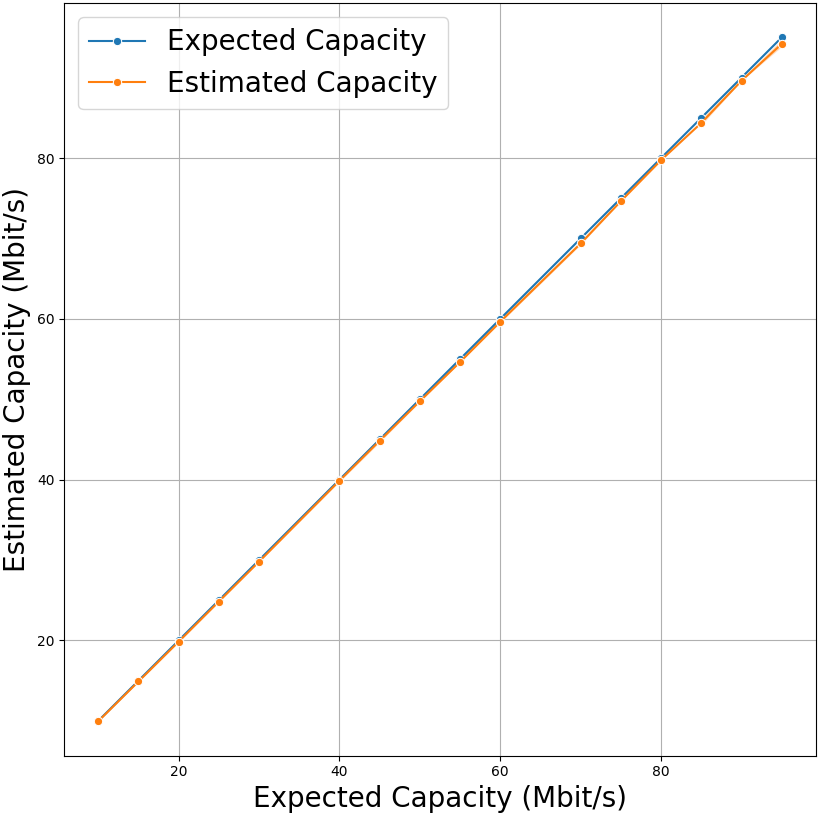
\includegraphics[width=.7\textwidth]{baseline_measurement}
 \caption{The baseline measurement results}
 \label{baseline}
\end{figure}

\begin{figure}[H]
 \centering
 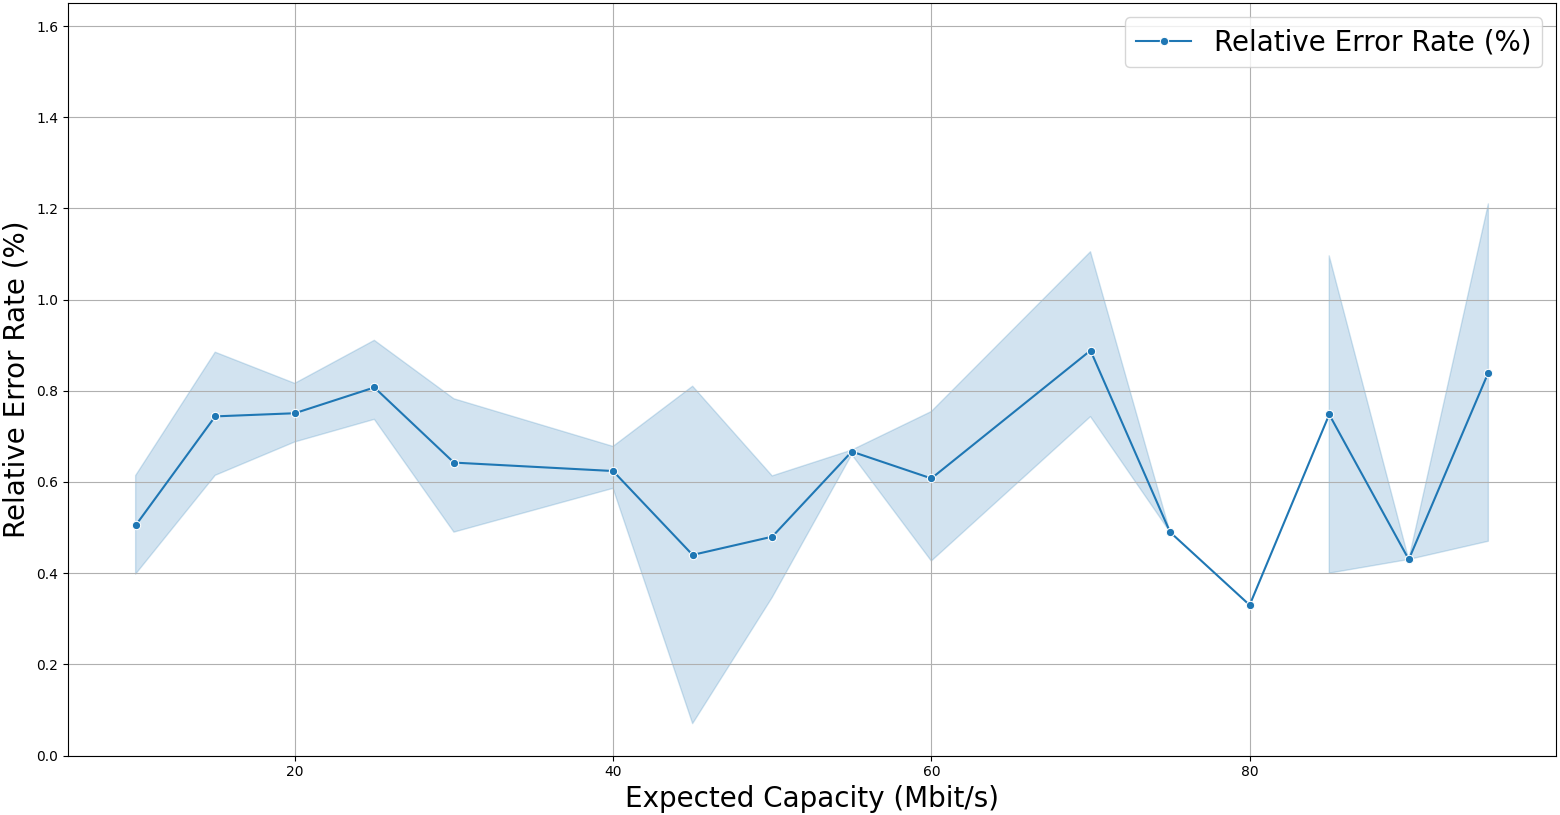
\includegraphics[width=\textwidth]{baseline_error}
 \caption{The baseline measurement error rate}
 \label{baseline_error}
\end{figure}

\begin{table}[H]
\centering
\begin{tabular}{ | m{11em} | m{1cm}| m{2cm} | } 
  \hline
  Average & 0.67\% \\ 
  \hline
  Standard Deviation & 0.27\% \\ 
  \hline
  Min Error & 0.07\% \\ 
  \hline
  Max Error & 1.55\% \\ 
  \hline
\end{tabular}
\caption{Relative error statistics of the baseline measurement}
\label{baseline_error_stats}
\end{table}

The baseline evaluation shows the the good potential of our approach, however it was conducted with the simplest and likely some of the most promising configuration possible, which is not likely to be the case in real networks.\\
In the next sections we will dissect each parameter through subsequent experiments and check their impact on the accuracy in order to evaluate how robust and useful our capacity estimation methodology can be in real life.  

\subsection{Path Length}
The first parameter to be analyzed is the path length from the source host to the sink, i.e. number of routers on the path. In order to analyze the impact that a path length can have on the measurement accuracy, we have to execute the test runs on different values of the given parameter. 

As the default TTL value in Linux for TCP and ICMP is 64\cite{ttl_hop_limit}, we decided to conduct measurements on arbitrary numbers of routers up to 63, namely 1, 3, 8, 20, 32 and 63. 
These numbers, although being chosen randomly apart from 1 and 63, paint a good picture of how our estimation tool reacts on networks with different sizes. Based on the results we can assume that the path length does not have an impact on the accuracy of our capacity estimation framework. Figures \ref{topo_size_3} and \ref{topo_size_63} depict the differences between actual and estimated capacity values on networks with path length of 3 and 63 respectively. (We chose to present only these two graphs, as there are practically no relevant differences between the results of different path lengths)

\begin{figure}[H]%[!tbp]
  \centering
  \begin{minipage}[b]{.45\textwidth}
    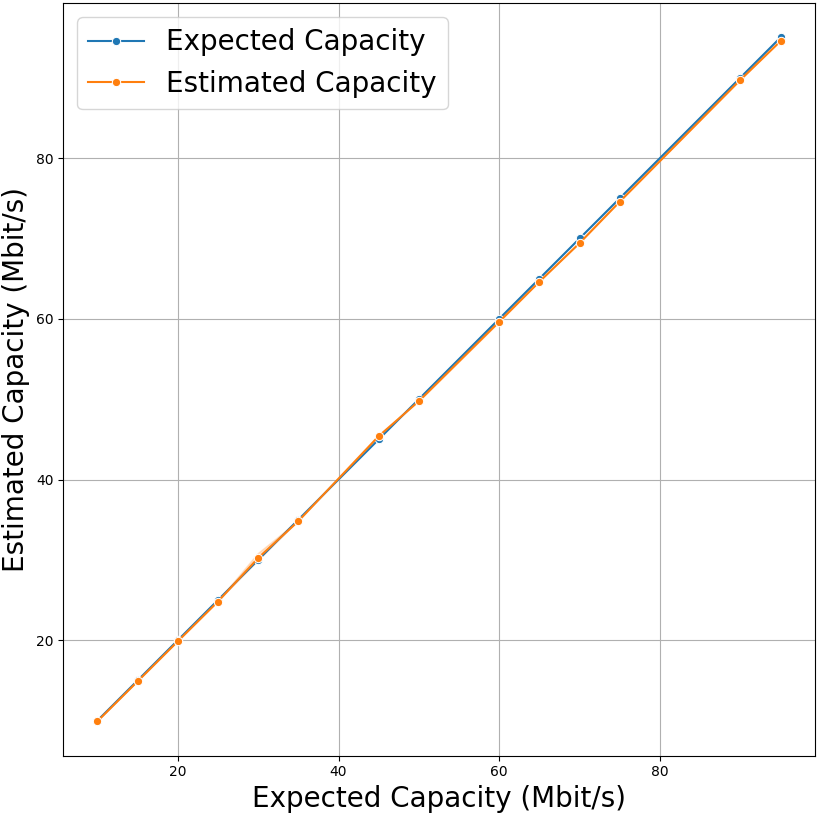
\includegraphics[width=\textwidth]{topo_size/topo_size_3}
    \caption{Path length: 3 Routers}
    \label{topo_size_3}
  \end{minipage}
  \hfill
  \begin{minipage}[b]{.45\textwidth}
    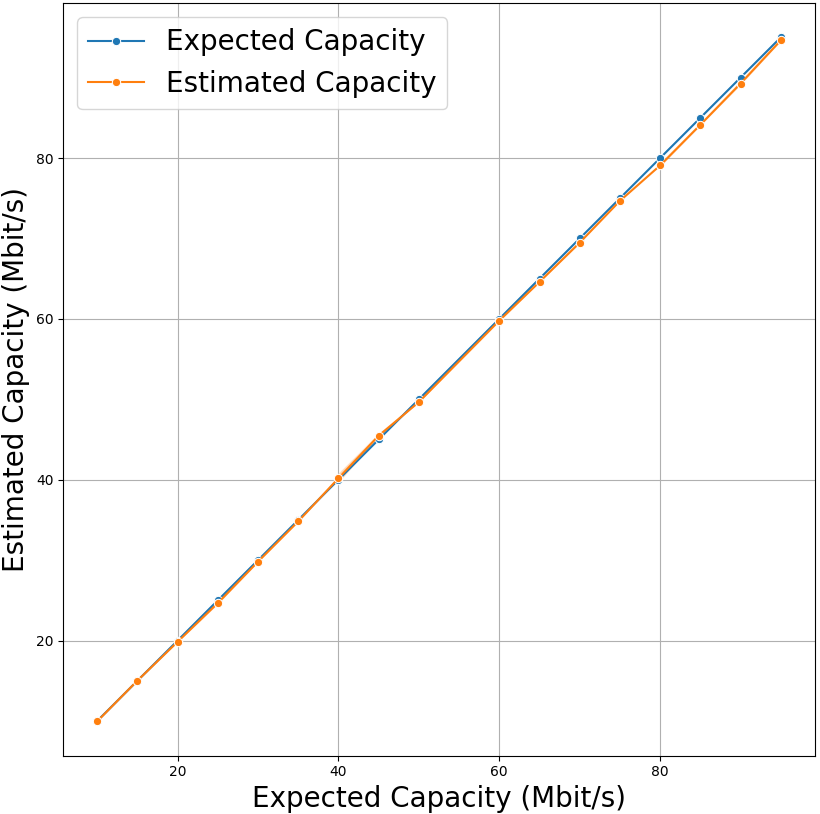
\includegraphics[width=\textwidth]{topo_size/topo_size_63}
    \caption{Path length: 63 Routers}
    \label{topo_size_63}
  \end{minipage}
\end{figure}

\begin{figure}[H]
 \centering
 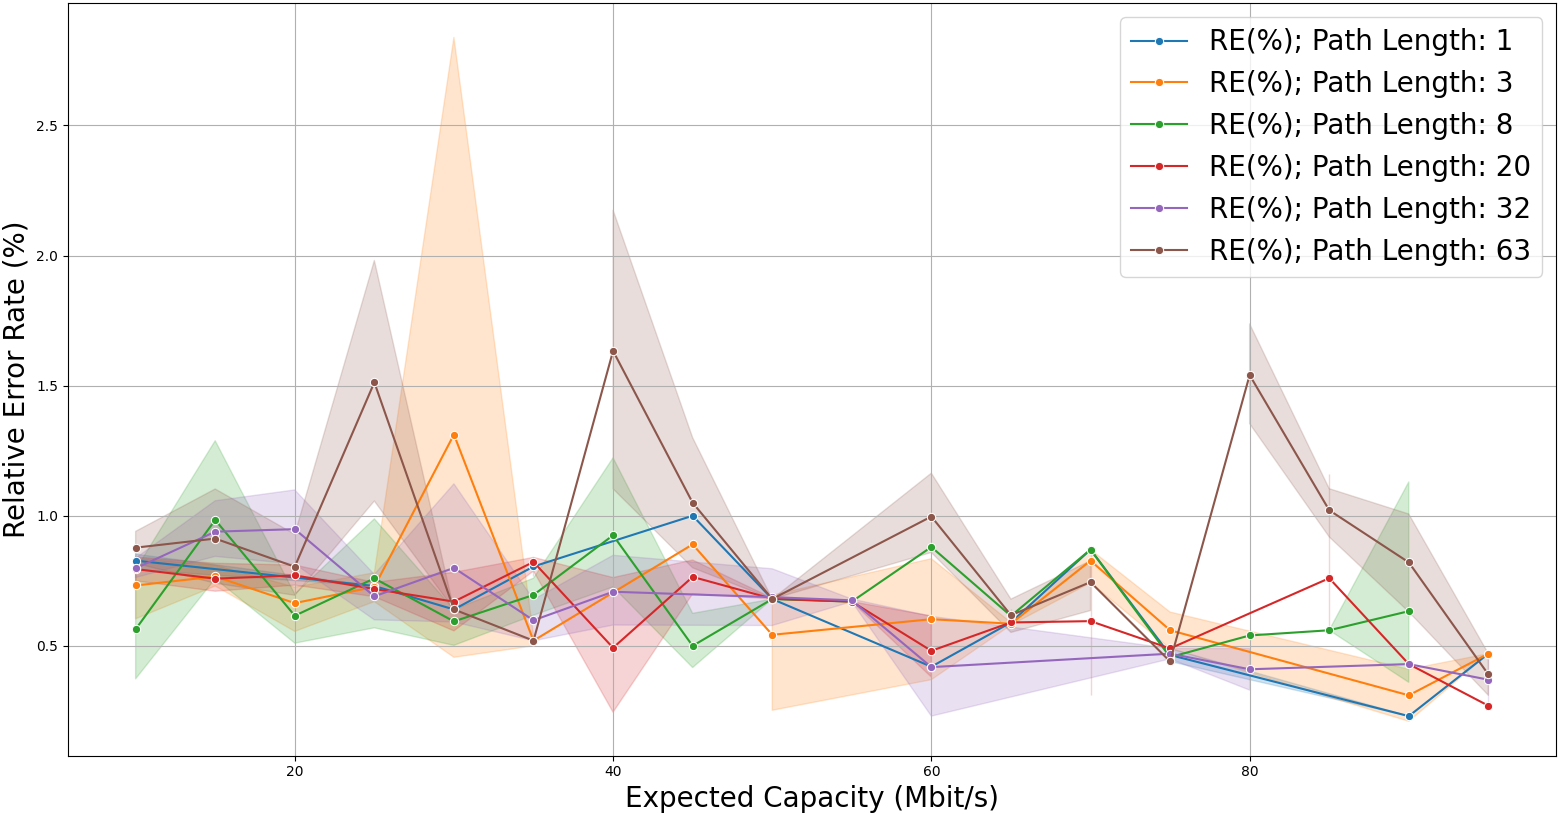
\includegraphics[width=\textwidth]{topo_size/topo_size_all_errors}
 \caption{Error rates on different path lengths}
 \label{topo_size_all_errors}
\end{figure}


The table \ref{plength_error_stats} depicts the comparison of relative error rates in more details and as one can observe, the differences are practically irrelevant. 


\begin{table}[h!]
  \centering
  \caption{Relative error stats of paths with different lengths.}
  \label{plength_error_stats}
\begin{tabular}{l|c|c|c|c|c}
\toprule
 Path Length & Average & Standard Deviation & Min Error & Max Error \\ \midrule
  \label{}
 1 	& 0.65\% & 0.21\% & 0.23\% & 1\% \\ 
 3 	& 0.72\% & 0.5\%  & 0.11\% & 4.3\% \\ 
 8 	& 0.74\% & 0.47\% & 0.01\% & 2.83\% \\
 20 & 0.75\% & 0.24\% & 0.01\% & 2.87\% \\
 32 & 0.83\% & 0.48\% & 0.0001\% & 4.09\% \\
 63 & 1.23\% & 2.53\% & 0.01\% & 42.57\% \\ \bottomrule
  \end{tabular}      
\end{table}



\subsection*{Conclusion}
Judging by the results of the experiments focusing on the path length conducted in an empty network we can conclude that the number of hops does not affect the accuracy of the estimation tool. At this point it can be safely assumed that when the cross-traffic is out of the picture, our framework can estimate capacity accurately no matter the amount of hosts on the path. Although there is still a small likelihood of major inaccuracies in measurements, such as $\approx$43\% relative error, it does not affect the overall picture, as it can be seen in the graphs.

After testing the path length we will further use 8 routers for the subsequent estimations as a default value.


\subsection{Packet Size}
Our next target parameter is the size of each packet in our generated traffic. 
As the packet size along with the amount of packets that have to be injected into the network can be the cause of the network overload, we have to find an optimal packet size that most importantly does not cost us the accuracy and also the load imposed on a target network remains minimal. In other words, the goal is to find the least packet size value that will deliver the accurate results.

We launched the tests with the packets of \ac{mtu} size, i.e. 1500 bytes and with the packets as small as 100 bytes. As depicted before, the former delivers highly accurate results, the latter, however, has shown an average relative error rate of $\approx$30\%, thus we decided to narrow down between the two values and find out at which packet size does relative error rate remain consistently low, i.e. what is the minimal packet size that matches the accuracy of 1500 bytes. 

\begin{figure}[t]
 \centering
 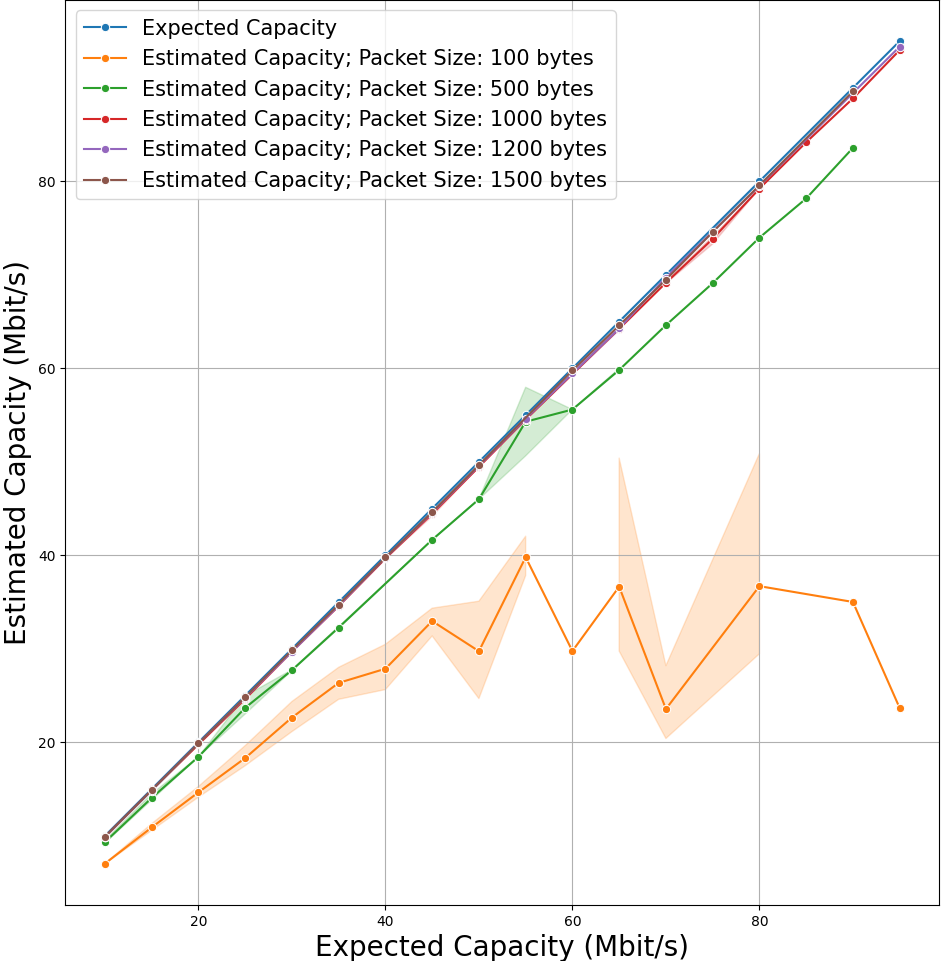
\includegraphics[width=.7\textwidth]{packet_size/packet_size_all}
 \caption{Comparison of the measurement results with different packet sizes}
 \label{packet_size_all}
\end{figure}


\begin{figure}[H]
 \centering
 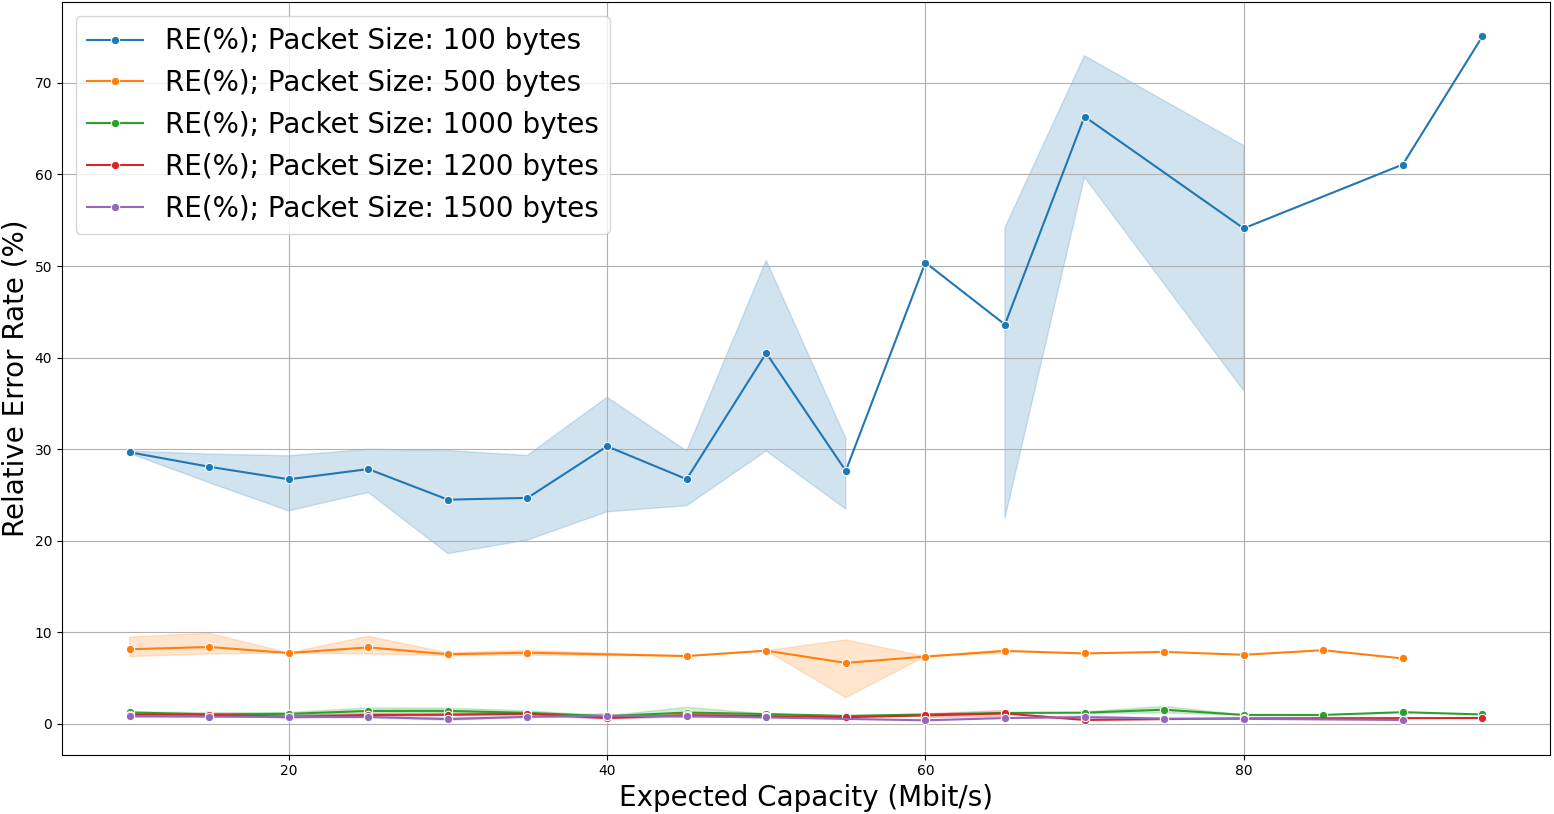
\includegraphics[width=\textwidth]{packet_size/packet_size_all_error}
 \caption{Error rates by packet size}
 \label{packet_size_all_error}
\end{figure}

Subsequently we tested packet sizes of 500, 1000 and 1200 bytes which showed drastic improvements in estimation accuracy. The results of these experiments are depicted in the figure \ref{packet_size_all} the respective error rates in the figure \ref{packet_size_all_error}. 


Depending on a researcher's threshold of the tolerable relative error rate the minimal packet size can vary. Thus we launched several more test runs with packet sizes between 500 and 1000 bytes in order to narrow down even more and to provide more detailed research. \\
The table \ref{packet_size_error_stats} shows the results of all the tests on packet size.

\begin{table}[h!]
  \centering
  \caption{Relative error rate statistics for packet size}
  \label{packet_size_error_stats}
\begin{tabular}{l|c|c|c|c|c}
\toprule
 Packet Size & Average & Standard Deviation & Min Error & Max Error \\ \midrule
  \label{}
    100  & 30.23\% & 10.97\% & 6.29\% & 75.24\% \\
    500  & 7.96\%  & 3.11\%  & 1.12\% & 41.57\% \\
    600  & 2.11\%  & 0.66\%  & 0.1\% & 4.85\% \\
    700  & 1.8\%   & 0.64\%  & 0.01\% & 5.92\% \\
    800  & 1.53\%  & 0.47\%  & 0.14\% & 4.6\% \\
    900  & 1.3\%   & 0.54\%  & 0.07\% & 5.42\% \\
    1000 & 1.15\%  & 0.48\%  & 0.0\% & 3.57\% \\
    1200 & 0.93\%  & 0.25\%  & 0.1\% & 1.72\% \\
    1500 & 0.77\%  & 0.32\%  & 0.13\% & 2.98\% \\ \bottomrule
  \end{tabular}      
\end{table}



\subsection*{Conclusion}
The estimations show that the impact of the packet size on the accuracy is huge and the packet size of 1500 bytes delivers the most accurate results. The accuracy declines along with the decreasing packet size. However, if we take, for example, less than 2\% as an average relative error rate that can be tolerated, we can decrease packet size down to 750 bytes (the half of the original 1500 bytes) and still get highly accurate results. \\
We should expect, though, that this number might not be sufficient in networks where the cross traffic is the case. This will be discussed in another section.



\subsection{Train Length}
In the original paper of PPrate\cite{pprate2006} En-Najjary and Urvoy-Keller state that the second version of the PPrate algorithm has good estimation results with as many as 300 IAT samples. Our previous estimations have also shown that the train length of 300 packets (299 IATs if packet loss is 0) can potentially be enough for accurate results with less than 1\% error rate.\\ But in this thesis we are aiming for the minimal intrusion. Therefore we are interested in decreasing the packet train lengths without compromising accuracy and finding out the least number of packets that will be provide the estimations as accurate as we have achieved with 300 packets.

The version of the Python implementation of PPrate by Brzoza\cite{Brzoza} that we are using for our estimations does not have a constraint on the amount of IAT samples. Thus we experimented on as small numbers of packets as possible. 

We conducted tests with different train lengths and the outcome was unexpected: The smallest train length that gave us accurate estimations was only 7 packets, meaning only 6 IATs were sufficient for PPrate to estimate capacity accurately. The algorithm was unable to calculate capacities with less than 6 IATs.  

Nevertheless there is one more factor to consider. In our experiments conducted in Mininet we could observe that the packet trains with less than 50 packets had almost no packet loss and increasing the train length often resulted in higher rate of loss without explicitly configuring packet loss. E.g. after 20 experiments with the trains of 7 packets the loss was 0.  

\begin{table}[h!]
  \centering
  \caption{Relative error statistics for packet train length}
  \label{train_length_error_stats}
\begin{tabular}{l|c|c|c|c|c}
\toprule
 Train Length & Average & Standard Deviation & Min Error & Max Error \\ \midrule
  \label{}
    7 & 1.42\% & 1.61\% & 0.01\% & 10.09\% \\
    10 & 1.25\% & 1.3\% & 0.03\% & 10.78\% \\
    20 & 1.1\% & 1.0\% & 0.05\% & 5.84\% \\
    50 & 0.81\% & 0.47\% & 0.01\% & 4.12\% \\
    100 & 0.78\% & 0.41\% & 0.03\% & 2.95\% \\
    250 & 0.74\% & 0.3\% & 0.07\% & 2.76\% \\ 
    500 & 0.53\% & 0.38\% & 0.05\% & 2.94\% \\
    1000 & 0.49\% & 0.43\% & 0.04\% & 3.39\% \\
    5000 & 0.42\% & 0.36\% & 0.02\% & 2.72\% \\ \bottomrule
  \end{tabular}      
\end{table}

The table \ref{train_length_error_stats} shows shows the statistics of relative error rate depending on the train length. It suggests that with the increase of the train length average error rate decreases, but the difference in estimation results between 7 packet train and 5000 packet train is only 1\%.

\subsection*{Conclusion}
The test results are showing that PPrate is able to provide high accuracy with a very small number of packets in a packet train when we are running tests on an empty network. Although more importantly it is notable that longer packet trains provide more accurate results. \\
These experiments, however, are not enough to assess that we can get the similar results in real networks where the cross-traffic is also an issue. This factor will be tested separately in section \ref{section_ct}. 




\subsection{Optimal Intrusion}
Based on our experiments on empty network we came to a conclusion that the packet size is more crucial parameter to the capacity estimation rather than packet train length. It is necessary that the packet size equals at least 700 bytes in order to keep the relative error rate reasonable, for example, below 2\% on average. \\
When it comes to the train length, however, the situation is more flexible here. Meaning, PPrate can deliver accurate results in empty network with as few as 10 packets. We combined these values and conducted the tests with 10 packet trains and 700 bytes packet size. It resulted in 3.36\% average relative error rate, therefore we increased both parameters several more times until the average error dropped below 2\%. \\
The table \ref{intrusion_error_stats} shows the results of those experiments. 

\begin{table}[h!]
  \centering
  \caption{Relative error statistics for optimal intrusion}
  \label{intrusion_error_stats}
\begin{tabular}{l|c|c|c|c|c|c}
\toprule
 Packet Size & Train Length & Average & Standard Deviation & Min Error & Max Error \\ \midrule
  \label{}
    700 & 10 & 3.36\% & 5.33\% & 0.04\% & 48.69\% \\
    700 & 50 & 2.19\% & 1.43\% & 0.08\% & 10.93\% \\
    800 & 10 & 6.7\% & 6.4\% & 0.01\% & 32.91\% \\
    800 & 30 & 1.81\% & 1.03\% & 0.11\% & 6.72\% \\
    1000 & 30 & 1.32\% & 0.44\% & 0.06\% & 3.75\% \\ \bottomrule
  \end{tabular}      
\end{table}


Assuming that real networks are not usually empty, we can hypothesize that in practice higher intrusion will be necessary for relatively precise estimations. We will further research this topic in section \ref{section_ct}

\subsection{Capacity Range}
One of the most important parameters is the capacity range of the links that we conduct our measurements on. So far we have seen that our tool can handle the links with capacities between 10 and 100 Mbits. The real networks can contain hops with higher capacities though, therefore it is necessary to research that aspect as well.

We tested the tool on several different networks with varying capacity ranges, such as [10, 100), as well as [100, 400), [400, 600) and [600, 1000) and as it appears, our methodology has a significant limitation when measuring the networks that contain links with relatively high capacities. 
Figures \ref{cap_range_all} and \ref{cap_range_all_error} show that the inaccuracy starts increasing with higher capacities.

\begin{figure}[h]
 \centering
 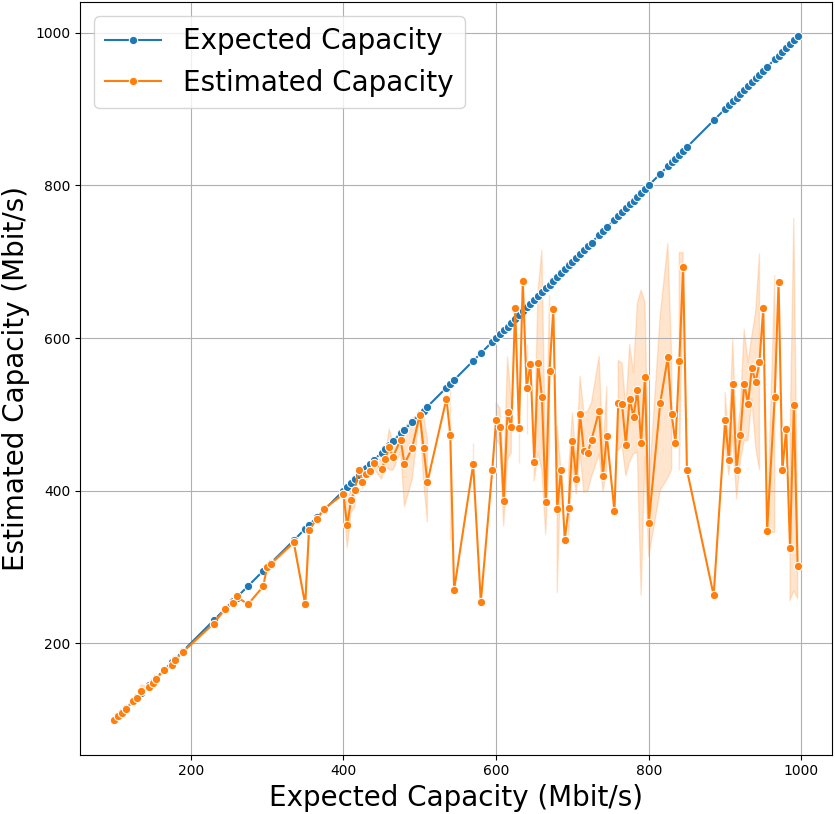
\includegraphics[width=.7\textwidth]{capacity_range/cap_range_100_1000}
 \caption{The impact of the capacity range on accuracy}
 \label{cap_range_all}
\end{figure}

\begin{figure}[H]
 \centering
 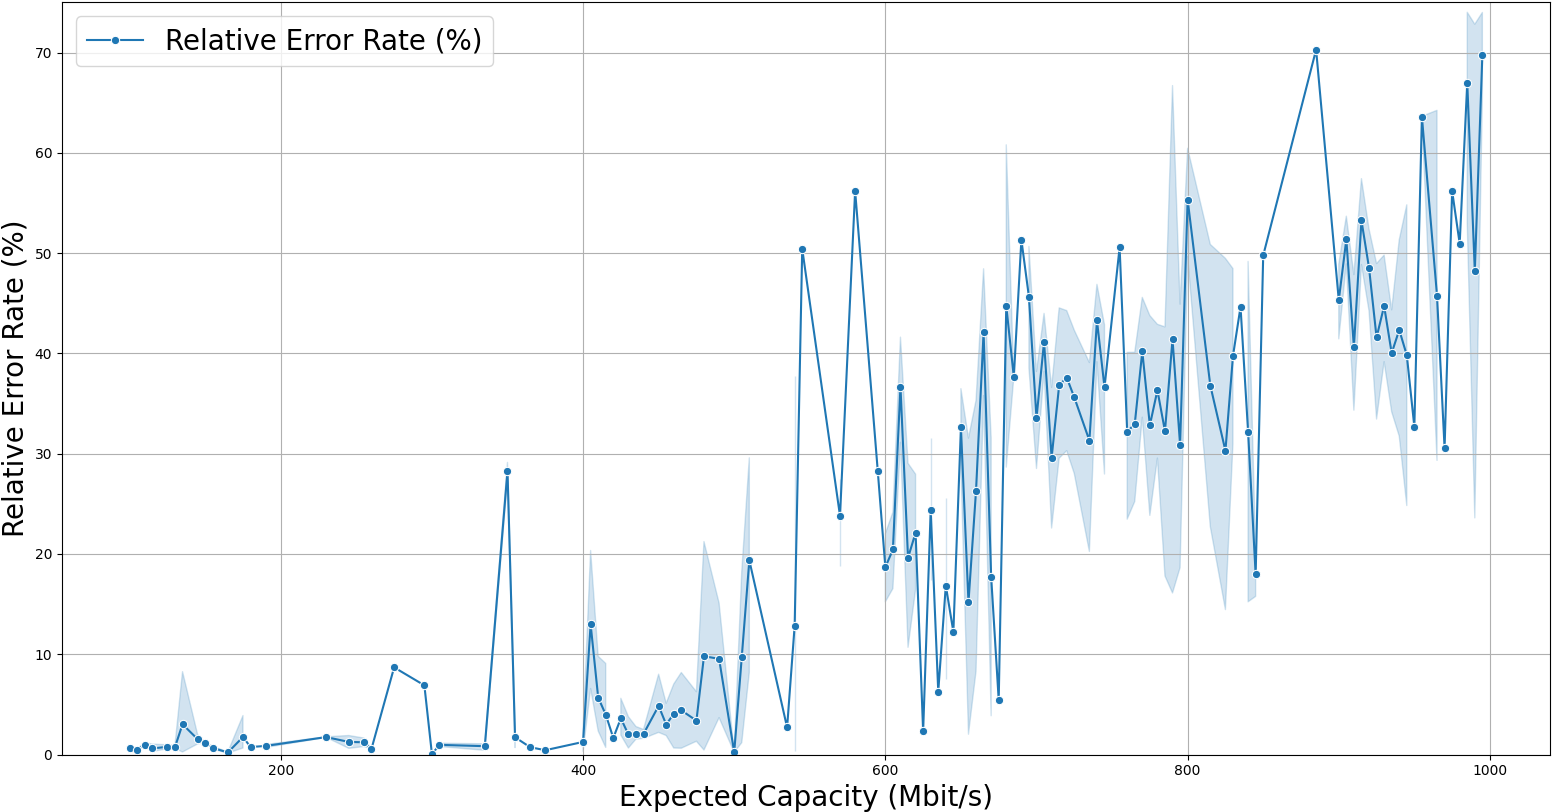
\includegraphics[width=\textwidth]{capacity_range/cap_range_100_1000_error}
 \caption{Error rates by capacity range}
 \label{cap_range_all_error}
\end{figure}




\subsection*{Conclusion}
In conclusion, we can deduce that the accuracy of the tool greatly depends on the capacity range. We can argue that on an empty network the accuracy is good for the paths that have the capacity value up to $\approx$250 Mbits. However the pattern emerges that capacities above 250 Mbits are not underestimated below 250. We can assume that the estimation results below 250 are accurate.
We will further observe this pattern with cross traffic in section \ref{section_ct}


\subsection{Packet Loss}
It is a very commonly occurred event in everyday internet traffic when data packets fail to reach their destination. This event is referred as packet loss and there can be different reasons that cause it. According to A. S. Gillis\cite{packet_loss_explained} it can be caused by overloaded network, software and/or hardware problems, etc.

\begin{figure}[h]
 \centering
 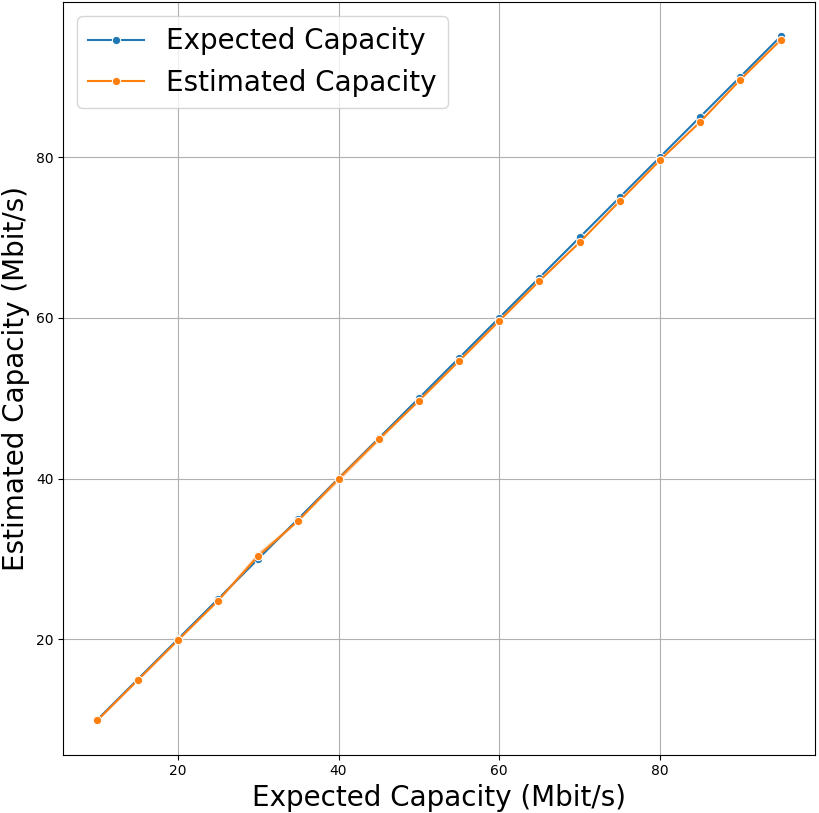
\includegraphics[width=.7\textwidth]{packet_loss/packet_loss}
 \caption{The impact of over 15\% packet loss on capacity estimation}
 \label{packet_loss_graph}
\end{figure}

 In order to make sure that our approach can cope with it and deliver the accurate estimations despite the lack of lost packets we tested our tool against this issue as well.
We chose the data samples where the total packet loss in each test run was above 15\%. These samples had on average 35\% total packet loss. Despite such a high loss the Figure \ref{packet_loss_graph} shows that the estimation accuracy was not compromised. 

According to the test results so far, we can assume that the random packet loss does not affect the accuracy to extent that affects accuracy, because most of the time it happens to the larger packet trains and the amounts of the ICMP packets that reach the source host is high enough for PPrate to estimate capacities precisely enough.
 
Although there is a special case of packet loss that represents a serious challenge to our estimation methodology, that is ICMP rate limiting. In contrast with the end-to-end estimation, during which the measurements are based on inter-arrival-times of TCP ack signals, ICMP messages are prone to a huge amount of packet loss due to the ICMP rate limits of internet routers.\\ 
We will further discuss this issue in the next section.


\subsection{ICMP Rate Limiting}
One of the biggest obstacles active ICMP-based measurement tools can face is ICMP rate limiting as it causes a huge rate of packet loss and also the packets that reach destination might not be suitable for capacity measurements. 
According to the Linux man page\cite{icmp_ratemask} it works in the following way: there are two parameters that have to be configured for ICMP rate control: \texttt{icmp\textunderscore ratemask} and \texttt{icmp\textunderscore ratelimit}. The first parameter consists of 19 bits each determining which types of ICMP should be affected by the rate limit (each bit corresponds to a specific ICMP type) and the second one sets the limit of the ICMP responses.
\texttt{icmp\textunderscore ratelimit} indicates the minimum time interval between ICMP responses and it is measured in milliseconds. The value range is [1, 1000]\cite{juniper} and in Linux it has a default value of 1000.

All of our previous measurements were conducted with disabled \texttt{icmp\textunderscore ratemask}. We have, however, also tested the effects of the rate limiting on our tool and tried to find out whether this can be a defining factor in the applicability of our methodology. 

As the Figure \ref{icmp_all} and the table \ref{icmp_error_stats} show the results are very unpredictable and unreliable.

\begin{figure}[H]
 \centering
 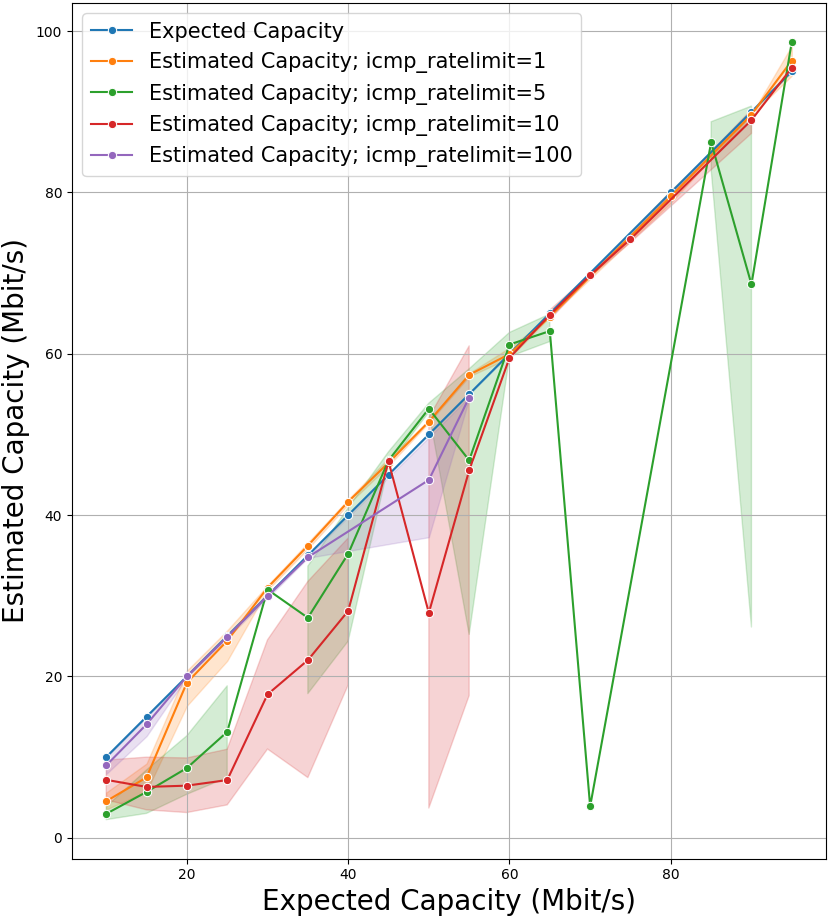
\includegraphics[width=0.7\textwidth]{icmp_ratelimit/icmp_all.png}
 \caption{Effects of ICMP rate limiting on the accuracy}
 \label{icmp_all}
\end{figure}


\begin{table}[h!]
  \centering
  \caption{Relative error statistics for the ICMP rate limiting}
  \label{icmp_error_stats}
\begin{tabular}{l|c|c|c|c|c}
\toprule
 Train Length & Average & Standard Deviation & Min Error & Max Error \\ \midrule
  \label{}
	1 & 22.19\% & 31.59\% & 0.02\% & 84.94\% \\
	5 & 50.45\% & 41.24\% & 0.1\% & 94.45\% \\
	10 & 48.24\% & 44.35\% & 0.13\% & 96.09\% \\
	100 & 5.79\% & 19.79\% & 0.06\% & 96.28\% \\ \bottomrule
  \end{tabular}      
\end{table}

Nevertheless we have made one observation, that resulted in some improvements in terms of accuracy: the increase in train length provided more accurate results, as despite the huge packet loss rate, the number of 'surviving' packets was high enough to drastically improve the accuracy rate. \\
The Figure \ref{icmp_1000} presents the results of the estimation with the train length of 5000 packets and \texttt{icmp\textunderscore ratelimit} of 1000 milliseconds.

\begin{figure}[H]
 \centering
 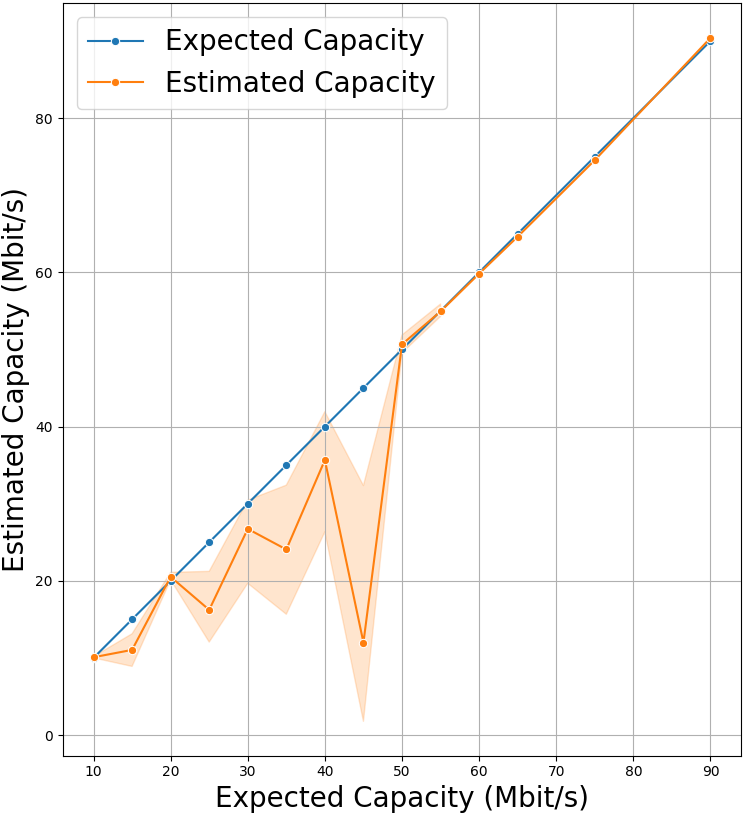
\includegraphics[width=0.7\textwidth]{icmp_ratelimit/icmp_1000_10k.png}
 \caption{The impact of long packet trains against ICMP rate limit}
 \label{icmp_1000}
\end{figure}


Further research is required to find better solutions to this important problem, which it is out of scope of this thesis, however there are some efforts made in this direction, namely the papers by Ravaioli et al. \cite{RaUrBa_icmp} and H. Guo and J. Heidemann\cite{fader2017}

\subsection{Summary}
To summarize this section, we have examined our capacity estimation technology in empty networks and tested it against different parameters. 
The results so far have shown that the tool provides high accuracy on any amount of hops with small packet trains and packet size of about 800 bytes. 
The tool has also shown some downsides, namely the inaccuracy is significant on high capacity networks and it is not reliable when the routers on the path have limits on ICMP response rates.

In the next section we will try to test our framework in a close to real life scenario, i.e. apply artificial cross traffic to each router on the path and observe its effects on accuracy.


\section{Evaluation during Cross-Traffic}
\label{section_ct}
We have conducted the previous experiments on empty networks without any cross-traffic. However this is not the case in the real Internet that we use on daily basis. 
Cross traffic seems to affect the test results significantly. 
What does 1.0 mean?
How our cross traffic works. - Formula of cross traffic

\subsection{Packet Size}

\subsection{Train Length}

\subsection{Optimal Intrusion during Cross-Traffic}

\subsection{Path Length}

\subsection{Capacity Range}

\subsection{Packet Loss}

\subsection{ICMP Rate Limiting}

\subsection{Summary}


\section{Data Replication}
One option to try to see if it can help
